\chapter{Prototype 1 Visualizations}
\label{prototype1Viz}

\begin{figure}[h!]
\centering
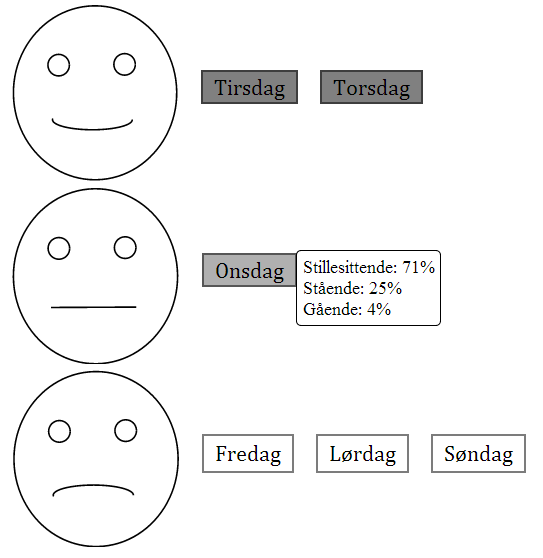
\includegraphics[totalheight=0.5\textheight, angle=-90]{u1First.png}
\caption[First version of U1]{First version of U1.}
\end{figure}

\begin{figure}[h!]
\centering
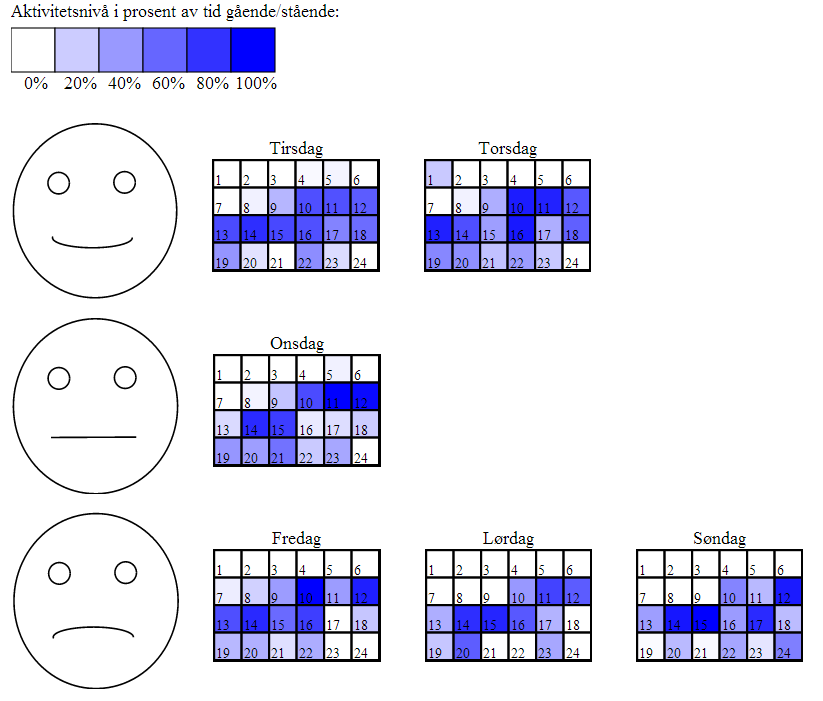
\includegraphics[totalheight=0.5\textheight, angle=90]{u2First.png}
\caption[First version of U2]{First version of U2.}
\end{figure}

\begin{figure}[h!]
\centering
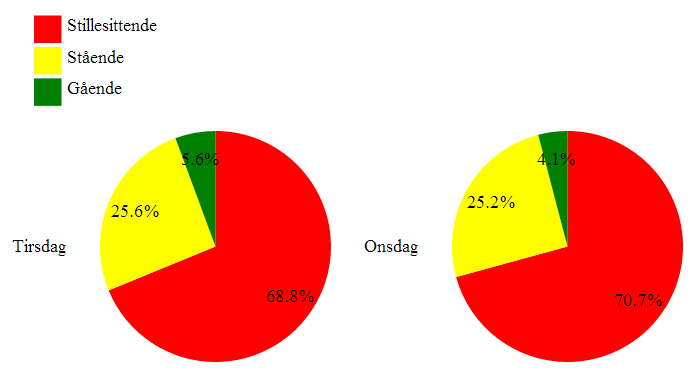
\includegraphics[totalheight=0.4\textheight, angle=-90]{f1First.png}
\caption[First version of F1]{First version of F1.}
\end{figure}

\begin{figure}[h!]
\centering
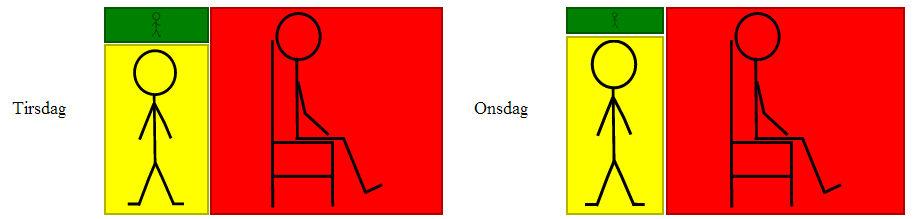
\includegraphics[totalheight=0.22\textheight, angle=90]{f2First.png}
\caption[First version of F2]{First version of F2.}
\end{figure}

\begin{figure}[h!]
\centering
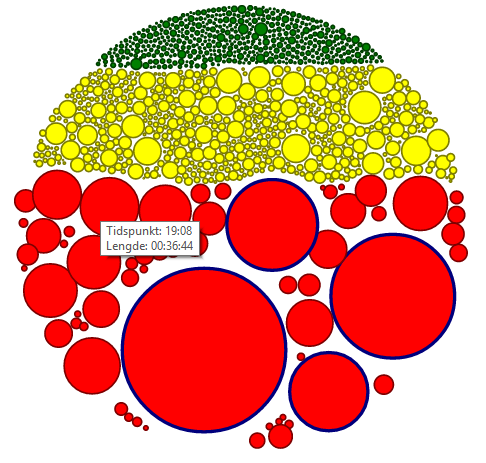
\includegraphics[totalheight=0.5\textheight, angle=-90]{f3First.png}
\caption[First version of F3]{First version of F3.}
\end{figure}

\begin{figure}[h!]
\centering
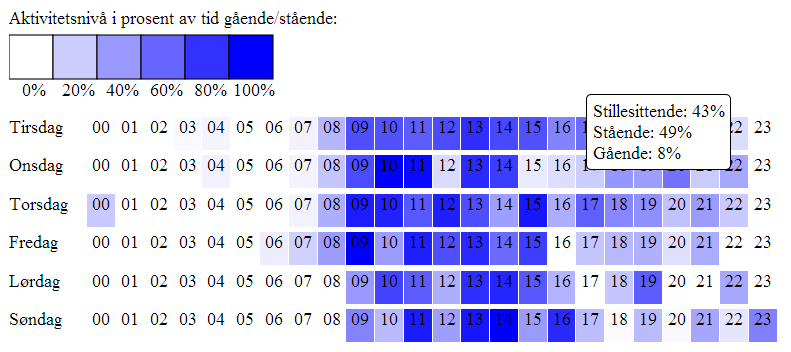
\includegraphics[totalheight=0.4\textheight, angle=90]{t1FirstWeek.png}
\caption[First version of T1]{First version of T1 in week overview.}
\end{figure}

\begin{figure}[h!]
\centering
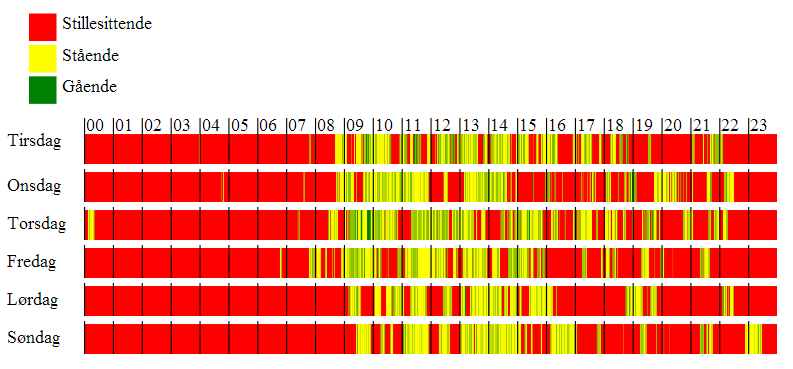
\includegraphics[totalheight=0.45\textheight, angle=-90]{t2FirstWeek.png}
\caption[First version of T2]{First version of T2 in week overview.}
\end{figure}

\begin{figure}[h!]
\centering
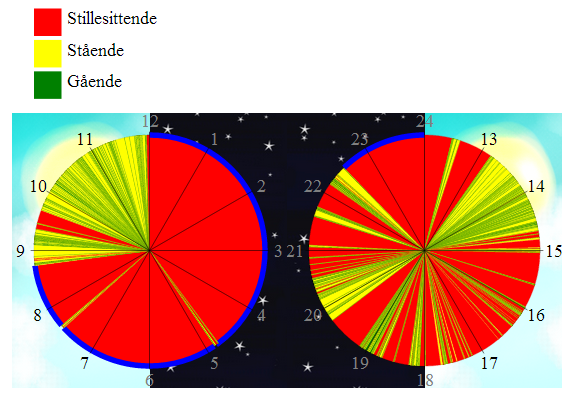
\includegraphics[totalheight=0.5\textheight, angle=90]{t3First.png}
\caption[First version of T3]{First version of T3}
\end{figure}

\begin{figure}[h!]
\centering
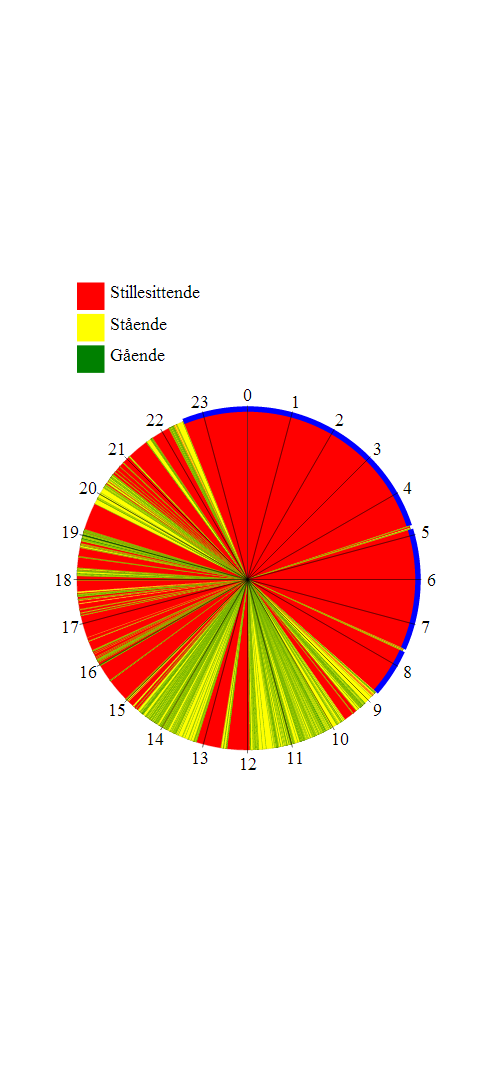
\includegraphics[totalheight=0.5\textheight, angle=-90]{t4First.png}
\caption[First version of T4]{First version of T4.}
\end{figure}

